\chapter{Inference for categorical data}
\label{inferenceForCategoricalData}

\section{Inference for a single proportion}
\label{singleProportion}


\subsection{Identifying when the sample proportion is nearly normal}\label{tenpercent}

A sample proportion can be described as a sample mean. If we represent each ``success'' as a 1 and each ``failure'' as a 0, then the sample proportion is the mean of these numerical outcomes:
\begin{eqnarray*}
\hat{p} = \frac{\ 0 + 1 + 1 + \cdots + 0\ }{1042} = 0.82
\end{eqnarray*}
The distribution of $\hat{p}$ is nearly normal when the distribution of 0's and 1's is not too strongly skewed for the sample size. The most common guideline for sample size and skew when working with proportions is to ensure that we expect to observe a minimum number of successes (1's) and failures (0's), typically at least 10 of each. The labels \term{success} and \term{failure} need not mean something positive or negative. These terms are just convenient words that are frequently used when discussing proportions.

\begin{termBox}{\tBoxTitle{Conditions for the sampling distribution of $\hat{p}$ being nearly normal}
The sampling distribution for $\hat{p}$, taken from a sample of size $n$ from a population with a true proportion $p$, is nearly normal when
\begin{enumerate}
\item the sample observations are independent and
\item we expected to see at least 10 successes and 10 failures in our sample, i.e. $np\geq10$ and $n(1-p)\geq10$. This is called the \term{success-failure condition}.
\end{enumerate}
If these conditions are met, then the sampling distribution of $\hat{p}$ is nearly normal with mean $p$ and standard error
\index{standard error (SE)!single proportion}
\begin{eqnarray}
\SE_{\hat{p}} = \sqrt{\frac{\ p(1-p)\ }{n}}
\label{seOfPHat}
\end{eqnarray}}
\end{termBox}\marginpar[\raggedright\vspace{-53mm}

$\hat{p}$\vspace{0mm}\\\footnotesize sample\\proportion\vspace{3mm}\\\normalsize$p$\vspace{0mm}\\\footnotesize population\\proportion]{\raggedright\vspace{-53mm}

$\hat{p}$\vspace{0mm}\\\footnotesize sample\\proportion\vspace{3mm}\\\normalsize$p$\vspace{0mm}\\\footnotesize population\\proportion}

Typically we don't know the true proportion, $p$, so we substitute some value to check conditions and to estimate the standard error. For confidence intervals, usually the sample proportion $\hat{p}$ is used to check the success-failure condition and compute the standard error. For hypothesis tests, typically the null value -- that is, the proportion claimed in the null hypothesis -- is used in place of $p$. Examples are presented for each of these cases in Sections~\ref{confIntForPropSection} and~\ref{htForPropSection}.



\subsection{Confidence intervals for a proportion}
\label{confIntForPropSection}

\index{point estimate!single proportion}

To verify that a sampling distribution of $\hat{p}$ is nearly normal we check:
\begin{description}
\item[Observations are independent.] For instance, we might be using a simple random sample and consist of fewer than 10\% of population, which verifies independence.
\item[Success-failure condition.] The sample size must also be sufficiently large, which is checked using the \hiddenterm{success-failure condition}. There are certain numbers of ``successes'' and ``failures'' in the sample, both greater than~10.
\end{description}
With the conditions met, we are assured that the sampling distribution of $\hat{p}$ is nearly normal. Next, a standard error for $\hat{p}$ is needed, and then we can employ the usual method to construct a confidence interval.

\begin{termBox}{\tBoxTitle[]{Constructing a confidence interval for a proportion}\vspace{-1mm}
\begin{itemize}
\setlength{\itemsep}{0mm}
\item Verify the observations are independent and also verify the success-failure condition using $\hat{p}$ and $n$.
\item If the conditions are met, the sampling distribution of $\hat{p}$ may be well-approximated by the normal model.
\item Construct the standard error using $\hat{p}$ in place of $p$ and apply the general confidence interval formula.\vspace{1mm}
\end{itemize}}
\end{termBox}


\begin{example}{Meta-confidence intervals?}
A student once asked, is there such a thing as a confidence interval for confidence intervals?
To answer this, let's step back and think about what is random and what is not. The confidence interval is a random interval; if you will, the left and right endpoints are two random variables $L$ and $R$.
In the long run, 95\% (or whatever confidence level we're working with) of these intervals will contain the parameter we are seeking confidence about. This parameter is not itself random, just unknown.
So instead of seeking meta-confidence, we may just study the distribution of $L$ and $R$.
\end{example}

\subsection{Hypothesis testing for a proportion}
	\label{htForPropSection}

	To apply the normal distribution framework in the context of a hypothesis test for a proportion, the independence and success-failure conditions must be satisfied. In a hypothesis test, the success-failure condition is checked using the null proportion: we verify $np_0$ and $n(1-p_0)$ are at least 10, where $p_0$ is the null value.

	\begin{termBox}{\tBoxTitle{Hypothesis test for a proportion}
	Set up hypotheses and verify the conditions using the null value, $p_0$, to ensure $\hat{p}$ is nearly normal under $H_0$. If the conditions hold, construct the standard error, again using $p_0$, and show the p-value in a drawing. Lastly, compute the p-value and evaluate the hypotheses.}
	\end{termBox}


\subsection{Thinking deeper about standard errors}
	When the null hypothesis says $p=1/2$, our score can be
	\[
		\frac{\hat p - 1/2}{\sqrt{\hat p(1-\hat p)/n}}
	\]
	but actually we may substitute $\hat p=1/2$ here in the denominator in order to be fair to the null hypothesis, as mentioned in \emph{OpenIntro Statistics}.

	When we do not assume $p_1=p_2$, our best (in some sense) guess for the standard error is
	\[
		\sqrt{\frac{\hat p_1(1-\hat p_1)}{n_1} + \frac{\hat p_2(1-\hat p_2)}{n_2}}
	\]
	This may be best in a maximum-likelihood sense (Chapter \ref{chMarkov}) but we should not expect it to be unbiased. For instance:
	\begin{exercise}
	\[
		\E(\hat p(1-\hat p)) = \left(1-\frac1n\right)(p-p^2)
	\]\footnote{To get started, rewrite $\hat p=\overline X$ and show that $\E((\overline X)^2) = \frac1n (p+(n-1)p^2)$.}
	\end{exercise}
	And indeed, it is clear that when $n=1$, $p(1-\hat p) = 0$ for both outcomes, and $\E(0)=0$.

	On the other hand, when we do assume $p_1=p_2$, the best estimate of $p_1$ and $p_2$ is
	\[
		\frac{p_1n_1+p_2n_2}{n_1+n_2}
	\]
	which is just the proportion obtained by pooling the samples together. 

	Note that if $n$ is small, a proportion $\hat p  = \frac1n\sum_{i=1}X_i$ with $X_i$ Bernoulli($p$) is in no way close to normal.
	Thus the $t$-distribution is never used in connection with proportions
	(it is only used when we have a small $n$ and $n$ is the number of independent normals available).
	When $n$ is large, we approximate a proportion using the normal distribution.


\subsection{Possible pitfall for pooled proportions}%Comment from the same class
When we're doing the standard error of $\hat p_1-\hat p_2$ under the assumption that $p_1=p_2$, we want to use the
pooled proportion $\hat p$ and then the standard error
\[
	\sqrt{\frac{\hat p(1-\hat p}{n_1}+\frac{\hat p(1-\hat p)}{n_2}}
\]
not just
\[
	\sqrt{\frac{\hat p(1-\hat p)}{n_1+n_2}}
\]
as the latter is the standard error of the pooled proportion $\hat p$, but we're interested in the difference $\hat p_1-\hat p_2$, not in what the (possibly same for both) proportion actually is!

In fact, a similar remark pertains to the case when we do not assume $p_1=p_2$. Consider Exercise \ref{gender_color_preference_CI_concept}. %Zain email
Let $p_y$ be the male proportion and $p_x$ female.
We need the standard error of $\hat p_y-\hat p_x$ which will be
\[
	\sqrt{\frac{\hat p_y(1-\hat p_y)}{1924}+\frac{\hat p_x(1-\hat p_x)}{3666}}.
\]

From this being 0.01 (since the width of the 95\%, hence $1.96\approx 2$ standard deviations, confidence interval is 0.02) and also $\hat p_y-\hat p_x=0.04$ we can deduce what they each are (Exercise \ref{zain_email}). One student in Fall 2018 instead considered $\hat p = \hat p_y-\hat p_x$ and then
$$\sqrt{\hat p(1-\hat p)/n}$$but this is treating $\hat p$ as a proportion. Note that $\hat p<0$ is possible, so $\hat p$ is not quite the same kind of beast as $\hat p_y$ and $\hat p_x$. 


\section{Difference of two proportions}
\label{differenceOfTwoProportions}

We would like to make conclusions about the difference in two population proportions: \mbox{$p_1 - p_2$}.

In our investigations, we first identify a reasonable point estimate of $p_1 - p_2$ based on the sample. You may have already guessed its form: $\hat{p}_1 - \hat{p}_2$\index{point estimate!difference of proportions}. Next, in each example we verify that the point estimate follows the normal model by checking certain conditions. Finally, we compute the estimate's standard error and apply our inferential framework.


\subsection{Sample distribution of the difference of two proportions}

We must check two conditions before applying the normal model to $\hat{p}_1 - \hat{p}_2$. First, the sampling distribution for each sample proportion must be nearly normal, and secondly, the samples must be independent. Under these two conditions, the sampling distribution of $\hat{p}_1 - \hat{p}_2$ may be well approximated using the normal model.

\begin{termBox}{\tBoxTitle{Conditions for the sampling distribution of $\hat{p}_1 - \hat{p}_2$ to be normal}
	The difference $\hat{p}_1 - \hat{p}_2$ tends to follow a normal model when
	\begin{itemize}
		\setlength{\itemsep}{0mm}
		\item each proportion separately follows a normal model, and
		\item the two samples are independent of each other.
	\end{itemize}
	The standard error of the difference in sample proportions is
	\index{standard error (SE)!difference in proportions}
	\begin{eqnarray}
		\SE_{\hat{p}_1 - \hat{p}_2}
			= \sqrt{\SE_{\hat{p}_1}^2 + \SE_{\hat{p}_2}^2}
			= \sqrt{\frac{p_1(1-p_1)}{n_1} + \frac{p_2(1-p_2)}{n_2}}
			\label{seForDiffOfProp}
	\end{eqnarray}
	where $p_1$ and $p_2$ represent the population proportions, and $n_1$ and $n_2$ represent the sample sizes.}
\end{termBox}

For the difference in two means, the standard error formula took the following form:
\begin{eqnarray*}
\SE_{\bar{x}_{1} - \bar{x}_{2}} = \sqrt{\SE_{\bar{x}_1}^2 + \SE_{\bar{x}_2}^2}
\end{eqnarray*}
The standard error for the difference in two proportions takes a similar form. The reasons behind this similarity are rooted in the probability theory of Section~\ref{randomVariablesSection}, which is described for this context in Guided Practice~\vref{derivingSEForDiffOfTwoMeansExercise}.


\subsection{Confidence intervals for $p_1 -p_2$}

In the setting of confidence intervals for a difference of two proportions, the two sample proportions are used to verify the success-failure condition and also compute the standard error, just as was the case with a single proportion.



\subsection{Hypothesis tests for $p_1 -p_2$}


\begin{termBox}{\tBoxTitle{Use the pooled proportion estimate when $\mathbf{H_0}$ is $\mathbf{p_1 - p_2 = 0}$}
When the null hypothesis is that the proportions are equal, use the pooled proportion ($\hat{p}$) to verify the success-failure condition and estimate the standard error:
\begin{eqnarray*}
\hat{p} = \frac{\text{number of ``successes''}}{\text{number of cases}} = \frac{\hat{p}_1n_1 + \hat{p}_2n_2}{n_1 + n_2}
\end{eqnarray*}
Here $\hat{p}_1n_1$ represents the number of successes in sample 1 since
\begin{eqnarray*}
\hat{p}_1 = \frac{\text{number of successes in sample 1}}{n_1}
\end{eqnarray*}
Similarly, $\hat{p}_2n_2$ represents the number of successes in sample 2.}
\end{termBox}


\subsection{More on 2-proportion hypothesis tests (special topic)}

When we conduct a 2-proportion hypothesis test, usually $H_0$ is $p_1 - p_2 = 0$. However, there are rare situations where we want to check for some difference in $p_1$ and $p_2$ that is some value other than 0. For example, maybe we care about checking a null hypothesis where $p_1 - p_2 = 0.1$.\footnote{We can also encounter a similar situation with a difference of two means, though no such example was given in Chapter~\ref{inferenceForNumericalData} since the methods remain exactly the same in the context of sample means. On the other hand, the success-failure condition and the calculation of the standard error vary slightly in different proportion contexts.} In contexts like these, we generally use $\hat{p}_1$ and $\hat{p}_2$ to check the success-failure condition and construct the standard error.

In a hypothesis test where the null hypothesis is that $p_1 - p_2 = 0.03$, say, the sample proportions $\hat p_1$ and $\hat p_2$ are used for the standard error calculation rather than a pooled proportion. Actually one could imagine using something like
\[
	\hat p(1-\hat p)/n_1 + (\hat p+0.03)(1-\hat p-0.03)/n_2\tag{*}
\]
Is using (*) a good idea?
In other words, are these unbiased, or maximum likelihood estimators, or minimum-variance?

Actually, (*) does not really make sense. If anything we should use $\hat p_1$ and $\hat p_1+0.03$, but then that ignores the information in the sample of size $n_2$.
The pooled $\hat p$ will give weight to one or the other depending on the relative sizes of $n_1$ and $n_2$, and so it does not make sense that it approximates $p_1$ in particular, or $p_2$ in particular.

\begin{example}{Curving exams.}\label{suspicious}
Suppose the pass rates for the course MATH 134 in 2008, 2009, 2010 are $.61$, $.63$, $.58$, respectively, and the grand passing rate overall is $.6$.
Suppose in 2009, $n=100$ students took the course. Is the passing rate of $.63$ suspiciously close to the overall passing rate of $.6$?
(Suspicion might arise that professors have decided approximately what they want the mean to be before the class even starts, regardless of how well students do.)
The standard error is
\[
	\frac{\sqrt{(0.6)(1-0.6)}}{\sqrt{100}} = \frac{\sqrt{.24}}{10} = .049 = 4.9\%.
\]
Our $Z$-score is
\[
	\frac{.63-.6}{.049} = \frac{.03}{.049} = \frac{30}{49}=0.61,
\]
and the probability of obtaining a value within $\pm 0.61$ of 0 for a standard normal distribution is calculated as

\sheets{=normdist(0.61,0,1,TRUE)-normdist(-0.61,0,1,TRUE)}%MAKE ALL SHEETS FORMULAS QUOTES

in Excel or Google Sheets which yields \texttt{0.458}. Thus, we do not reject the null hypothesis that 2009 was a year that just followed a normal distribution with mean 0.6; we do not have evidence of excessive curving.

Let us construct an example where curving does seem to have happened. Suppose in 2008, $\hat p_1=.601$, with $n_1=1000$.
Then suppose in 2009, $\hat p_2=.599$, with $n_2=1000$ as well.
Now we can use $p=.6$ as our grand proportion (estimated). The $Z$-score for a particular year, say 2008, is
\[
	\frac{.601-.6}{\sqrt{(.6)(1-.6)/1000}} = \frac{.001}{\sqrt{1/240}} = \sqrt{240}/1000 = \sqrt{2.4}/100 = 0.0155
\]
and the probability that a standard normal random variable $Z$ will have $|Z|\le 0.0155$ is quite small.
If each year has a small $p$-value like this, we can be quite sure that curving occurs.
If none of them do, we can be quite sure it doesn't.
If some do and some don't, we are getting into a more subtle area: the ones that did may have just done so by coincidence.


Now let us try to construct an example for means rather than proportions.
Suppose in 2008 the mean grade point (the grade point for A is 4, for A- is 3.7, for B+ is 3.3, for B is 3, and so on) is 2.9 with 100 students and a sample standard deviation in the grade points of 1.0 (a reasonable number that is sometimes, in fact, used by instructors to ``curve the standard deviation'').
Suppose in 2009, the mean grade point was 3.0, with the same number of students and sample standard deviation.
Is this suspicious?
If the true mean, in some sense, is 2.95, what is the $Z$-score for an observation of 3.0?
Since the standard deviation is 1, an individual observation of 3.0 (a single B grade) is 0.05 standard deviations from the mean:
The code is
\sheets{=normdist(0.05,0,1,TRUE)-normdist(-0.05,0,1,TRUE)}
which gives 4.0\%. This might be suspicious if the class had just one student.

If 3.0 is the mean for a whole class of 100 students, the $Z$-score is
\[
	\frac{3.0-2.95}{s/\sqrt{n}} = \frac{0.05}{1/10} = 0.15
\]
As $n$ gets large, we expect the means to have smaller standard deviations, which means that a mean close to the true mean $\mu$ becomes less and less suspicious.
But suppose that while the standard deviation of the individual grades is 1, the means are 2.951 in 2008 and 2.949 in 2009.
Then assuming the true mean is 2.95, the $Z$-score of 2.951 is
\[
	\frac{2.951-2.95}{1/10} = .01
\]
which gives a $p$-value 0.007978712629 via

\sheets{=normdist(0.01,0,1,TRUE)-normdist(-0.01,0,1,TRUE)}

The problem now is that the only way to get the means that close together (without making them actually equal) may be to increase the sample size; so let us try to make a more specific example.
Since grade points are at least 0.3 apart, the sum of grade points in a class must be an integer multiple of 0.1. Thus in a class of $10^k$ students, the mean is an integer multiple of $10^{-(k+1)}$.
On the other hand $\sqrt{10^k}=10^{k/2}$ so the $Z$-score (when the grand mean is an integer, say) must be an integer multiple of $10^{k/2-k-1}$. When $k=2$ this is $10^{-2}$. As $k\to\infty$ this does go to zero, meaning that we can make meaningful checks for curving.
\end{example}


\section{Testing for goodness of fit using \texorpdfstring{$\chi^2$}{chi-square}}
\label{oneWayChiSquare}


Sometimes we don't want to investigate a single parameter, but a whole distribution. Say you have a random variable $X$ which takes values in $\{0,\dots,k\}$ with certain probabilities $p_0,\dots,p_k$.
Now you draw $n$ sample values and observe $O_i$ many times that $X=i$. The expected number of times to observe $X=i$ would be $np_i$. So if $|O_i-np_i|$ is large we should reject the null hypothesis that the data were drawn from the suspected distribution given by the $p_i$. The $\chi^2$-statistic gives us a way to package the numbers $|O_i-np_i|$ for $0\le i\le k$ into a single number for this hypothesis testing task.

We do not study confidence intervals in this setting, although it could be an intriguing idea (imagine a ``tube'' around the histogram for our probability distribution, showing how sure we are about the values $p_i$).


\subsection{The $\chi^2$ test statistic}
\label{chiSquareTestStatistic}

Squaring here enables a connection with normal random variables. In fact a $\chi^2$ random variable with $n$ degrees of freedom is $\sum_{i=1}^n Z_i^2$ where $Z_i$ are independent standard normal random variables.

The test statistic $\chi^2$\marginpar[\raggedright\vspace{9mm}

$\chi^2$\vspace{0.5mm}\\\footnotesize chi-square\\test statistic]{\raggedright\vspace{9mm}

$\chi^2$\vspace{0.5mm}\\\footnotesize chi-square\\test statistic},\index{chi-square statistic} which is the sum of the $Z^2$ values, is generally used for these reasons. We can also write an equation for $\chi^2$ using the observed counts and null counts:
%\index{data!racial make-up of jury|)}
{\begin{align*}
\chi^2 &= \sum_{i=1}^{\#\text{counts}}
	\frac
	{\text{\footnotesize$(\text{observed count}_i - \text{null count}_i)^2$}}
	{\text{\footnotesize$\text{null count}_i$}}
\end{align*}
}The final number $\chi^2$ summarizes how strongly the observed counts tend to deviate from the null counts. In Section~\ref{pValueForAChiSquareTest}, we will see that if the null hypothesis is true, then $\chi^2$ follows a new distribution called a \emph{$\chi^2$ distribution}. Using this distribution, we will be able to obtain a p-value to evaluate the hypotheses.


\subsection{The $\chi^2$ distribution and finding areas}

The \term{$\chi^2$ distribution} is sometimes used to characterize data sets and statistics that are always positive and typically right skewed. Recall the normal distribution had two parameters -- mean and standard deviation -- that could be used to describe its exact characteristics. The $\chi^2$ distribution has just one parameter called \termsub{degrees of freedom (df)}{degrees of freedom (df)!chi-square}, which influences the shape, center, and spread of the distribution.


\begin{figure}%[h]
\centering
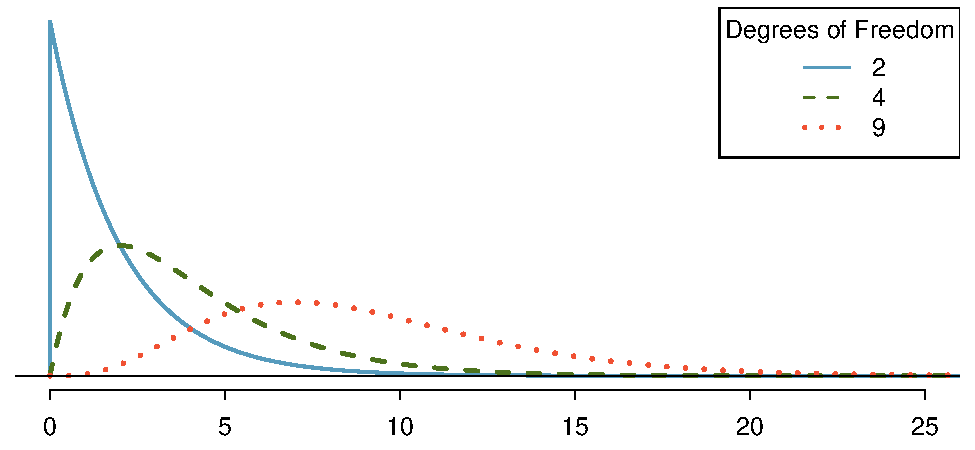
\includegraphics[width=0.9\textwidth]{ch_inference_for_props/figures/chiSquareDistributionWithInceasingDF/chiSquareDistributionWithInceasingDF}
\caption{Three $\chi^2$ distributions with varying degrees of freedom.}
\label{chiSquareDistributionWithInceasingDF}
\end{figure}


Our principal interest in the $\chi^2$ distribution is the calculation of p-values, which (as we have seen before) is related to finding the relevant area in the tail of a distribution. To do so, a new table is needed: the \term{$\chi^2$ table}, partially shown in Table~\ref{chiSquareProbabilityTableShort}.

Note that we only consider 1-sided tests, where the area of the right tail is of interest. This is because there is only one way to get an extreme result: a large value for the $\chi^2$ statistic. In the normal case we could get a positive or negative result, leading to subtleties related to 1-sidedness and 2-sidedness. The left ``tail'' would only be of interest if we were testing whether the fit is suspiciously good as in Example \ref{suspicious}.

\begin{table}%[h]
\centering
\begin{tabular}{r | rrrr | rrrr |}
  \hline
Upper tail & 0.3 & 0.2 & 0.1 & 0.05 & 0.02 & 0.01 & 0.005 & 0.001 \\ 
  \hline
%df \hfill 1 & \footnotesize 1.07 & \footnotesize 1.64 & \footnotesize 2.71 & \footnotesize 3.84 & \footnotesize 5.41 & \footnotesize 6.63 & \footnotesize 7.88 & \footnotesize 10.83 \\ 
df \hfill 2 & \footnotesize 2.41 & \footnotesize \highlightO{3.22} & \footnotesize \highlightO{4.61} & \footnotesize 5.99 & \footnotesize 7.82 & \footnotesize 9.21 & \footnotesize 10.60 & \footnotesize 13.82 \\ 
  \em3 & \em\footnotesize 3.66 & \em\footnotesize 4.64 & \em\footnotesize \highlightT{6.25} & \em\footnotesize 7.81 & \em\footnotesize 9.84 & \em\footnotesize 11.34 & \em\footnotesize 12.84 & \em\footnotesize 16.27 \\ 
  4 & \footnotesize 4.88 & \footnotesize 5.99 & \footnotesize 7.78 & \footnotesize 9.49 & \footnotesize 11.67 & \footnotesize 13.28 & \footnotesize 14.86 & \footnotesize 18.47 \\ 
  5 & \footnotesize 6.06 & \footnotesize 7.29 & \footnotesize 9.24 & \footnotesize 11.07 & \footnotesize 13.39 & \footnotesize 15.09 & \footnotesize 16.75 & \footnotesize 20.52 \\ 
  \hline
  6 & \footnotesize 7.23 & \footnotesize 8.56 & \footnotesize 10.64 & \footnotesize 12.59 & \footnotesize 15.03 & \footnotesize 16.81 & \footnotesize 18.55 & \footnotesize 22.46 \\ 
  7 & \footnotesize 8.38 & \footnotesize 9.80 & \footnotesize 12.02 & \footnotesize 14.07 & \footnotesize 16.62 & \footnotesize 18.48 & \footnotesize 20.28 & \footnotesize 24.32 \\ 
  \hline
\end{tabular}
\caption{A section of a $\chi^2$ table.}
\label{chiSquareProbabilityTableShort}
\end{table}

\textC{\pagebreak}


\subsection{Finding a p-value for a $\chi^2$ distribution}
\label{pValueForAChiSquareTest}


\begin{termBox}{\tBoxTitle{Chi-square test for one-way table}
Suppose we are to evaluate whether there is convincing evidence that a set of observed counts $O_1, O_2, \dots, O_k$ in $k$ categories are unusually different from what might be expected under a null hypothesis. Call the \emph{expected counts} that are based on the null hypothesis $E_1, E_2, \dots, E_k$. If each expected count is at least 5 and the null hypothesis is true, then the test statistic below follows a $\chi^2$ distribution with $k-1$ degrees of freedom:
\begin{align*}
\chi^2 = \frac{(O_1 - E_1)^2}{E_1} + \frac{(O_2 - E_2)^2}{E_2} + \cdots + \frac{(O_k - E_k)^2}{E_k}
\end{align*}
The p-value for this test statistic is found by looking at the upper tail of this $\chi^2$ distribution. We consider the upper tail because larger values of $\chi^2$ would provide greater evidence against the null hypothesis.}
\end{termBox}

\begin{tipBox}{\tipBoxTitle{Conditions for the $\chi^2$ test}
There are two conditions that must be checked before performing a $\chi^2$ test:\vspace{-1mm}
\begin{description}
\setlength{\itemsep}{0mm}
\item[Independence.] Each case that contributes a count to the table must be independent of all the other cases in the table.
\item[Sample size / distribution.] Each particular scenario (i.e. cell count) must have at least 5~expected cases.
\vspace{-1mm}
\end{description}
Failing to check conditions may affect the test's error rates.}
\end{tipBox}

When examining a table with just two bins, pick a single bin and use the one-proportion methods introduced in Section~\ref{singleProportion}.

\section{Testing for independence in two-way tables}
\label{twoWayTablesAndChiSquare}

\begin{termBox}{\tBoxTitle{Computing expected counts in a two-way table}
To identify the expected count for the $i^{th}$ row and $j^{th}$ column, compute
\[
	\text{Expected Count}_{\text{row }i,\text{ col }j} = \frac{(\text{row $i$ total}) \times  (\text{column $j$ total})}{\text{table total}}\vspace{2mm}
\]
}
\end{termBox}


%\textC{\newpage}


\subsection{The $\chi^2$ test for two-way tables}

\begin{termBox}{\tBoxTitle{Computing degrees of freedom for a two-way table}
When applying the $\chi^2$ test to a two-way table, we use
$$ df = (R-1)\times (C-1) $$
where $R$ is the number of rows in the table and $C$ is the number of columns.}
\end{termBox}

\begin{tipBox}{\tipBoxTitle{Use two-proportion methods for 2-by-2 contingency tables}
When analyzing 2-by-2 contingency tables, we end up with 1 degree of freedom, i.e., $Z^2$ where $Z$ is standard normal. So then we use the two-proportion methods introduced in Section~\ref{differenceOfTwoProportions}.}
\end{tipBox}

\begin{figure}%[h]
\centering
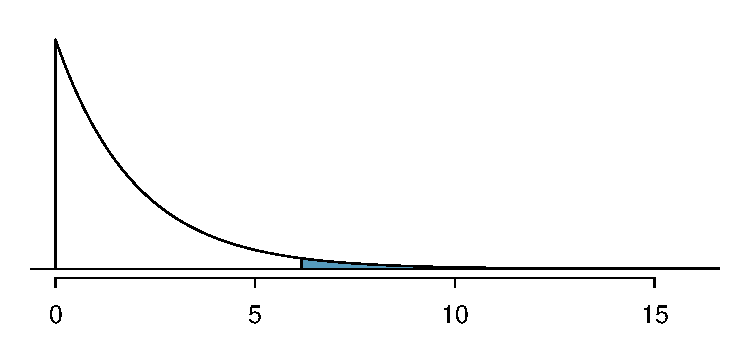
\includegraphics[width=0.7\textwidth]{ch_inference_for_props/figures/googleHTForDiffAlgPerformancePValue/googleHTForDiffAlgPerformancePValue}
\caption{A $p$-value represented as an area under the curve of the pdf for a $\chi^2$ with 2 df.}
\label{googleHTForDiffAlgPerformancePValue}
\end{figure}


\subsection{The $\chi^2$ distribution with 1 degree of freedom}

For $a\ge 0$,
\begin{eqnarray*}
	F(a) = \P(Z^2\le a) &=& \P(-\sqrt{a}\le Z\le\sqrt{a}) \\
	&=& \P(Z\le\sqrt{a})-\P(Z\le-\sqrt{a})\\
	&=& \Phi(\sqrt{a}) - (1-\Phi(\sqrt{a}))\\
	&=& 2\Phi(\sqrt{a})-1;\\
	f(a) &=& 2f_Z(\sqrt{a})\cdot \frac1{2\sqrt{a}} = \frac1{\sqrt{a}}\cdot\frac1{\sqrt{2\pi}} e^{-a/2}.
\end{eqnarray*}
Note that
\[
	\lim_{a\to 0^+} f(a) = \frac1{0\cdot 1}=+\infty.
\]
so the pdf has a vertical asymptote at $0$.

For 2 degrees of freedom, we would have to consider
\[
	\P(Z_1^2+Z_2^2\le a)=\iint\dots
\]
which is done in advanced courses (that assume knowledge of multivariable calculus).
Would we use $\chi^2(1)$ for flipping a coin?
Let $X$ be binomial with parameters $n$ and $p$, then
\[
	\chi^2 = \frac{(X-np)^2}{np} + \frac{(n-X-n(1-p))^2}{n(1-p)} = \left(\frac{X-np}{\sqrt{np(1-p)}}\right)^2
\]
so using $\chi^2$ in this case would be no different from using the binomial approximation to the normal distribution.
\begin{exercise}
	Verify the computation just made.\footnote{The intermediate step is
	\[
		\frac{(X-np)^2(1-p)+(np-X)^2p}{np(1-p)}.
	\]}
\end{exercise}